\chapter{Implementacija i korisničko sučelje}
		
		
		\section{Korištene tehnologije i alati}
		
			Komunikacija u timu izvedena je putem dva servisa. Korištenjem aplikacije WhatsApp\footnote{https://www.whatsapp.com/}, te na serveru u aplikaciji Discord\footnote{https://discord.com/}. Oboje imaju mogućnosti grupnih poziva, dijeljena ekrana te slanja poruka u grupni \textit{chat}. 
			Za izradu UML dijagrama u dokumentaciji korištena je aplikacija Astah\footnote{https://astah.net/} UML kompanije ChangeVision\footnote{https://www.change-vision.com/}. Za kontrolu verzija izvornog koda korišten je Git\footnote{https://git-scm.com/}, a kao udaljeni repozitorij svog koda i dokumentacije korišten je direktorij na web platformi GitHub\footnote{https://github.com/}.
			Kao razvojno okruženje koristili smo IntelliJ IDEA\footnote{https://www.jetbrains.com/idea/}, integrirano razvojno okruženje (IDE) proizvedeno od strane JetBrains\footnote{https://www.jetbrains.com/}. IntelliJ IDEA koristi se za razvoj aplikacija pisanih u Javi\footnote{https://www.java.com/en/}, Kotlin-u\footnote{https://kotlinlang.org/}, Groovy-u\footnote{https://groovy-lang.org/} i drugim JVM baziranim programskim jezicima.
			Aplikacija je napisana u Java programskom jeziku koristeči alat \textit{Spring Boot}\footnote{https://spring.io/projects/spring-boot/} za razvoj \textit{backenda}, a za razvoj \textit{frontenda} korišten je React\footnote{https://react.dev/}. React je biblioteka programskog jezika JavaScript\footnote{https://www.javascript.com/}, koja se koristi za razvoj programskih sučelja, a stvorio ju je i održava Meta\footnote{https://about.meta.com/}. \textit{Spring Boot} alat je Spring\footnote{https://spring.io/} Framework-a, koji je aplikacijski \textit{framework} za razvoj Java aplikacija, najčešće onih baziranih na rad na web-u.
			Grafički dizajn \textit{frontend} dijela aplikacije rađen je u alatu Powerpoint\footnote{https://www.microsoft.com/hr-hr/microsoft-365/powerpoint} proizvođača Microsoft\footnote{https://www.microsoft.com/hr-hr/}.
			Za bazu podataka koristili smo H2\footnote{https://www.h2database.com/html/main.html}, koji je prilagođen radu u Javi i baziran na poslužitelju, za kojeg smo odabrali Render\footnote{https://render.com/}. Prilikom testiranja POST i GET metoda koristili smo se alatom Postman\footnote{https://www.postman.com/}.
			
			\eject 
		
	
		\section{Ispitivanje programskog rješenja}
			\subsection{Ispitivanje komponenti}
			\text Prilikom ispitivanja komponenti izveden je 21 test nad razredima u izvornom kodu. Ovo potpoglavlje biti će ograničeno na svega 6, no ostale je moguće vidjeti na GitHub repozitoriju. Poveznica na isti nalazi se u literaturi. Također, bitno je spomenuti da se sekcija testova naziva \textit{DoctorControllerTest} može gledati kao skupina koja se odnosi i na korisnike tipa Pedijatar i korisnike tipa Liječnik obiteljske medicine, zbog sličnosti izvedbe razreda.
			
			%unos slike
			\begin{figure}[H]
				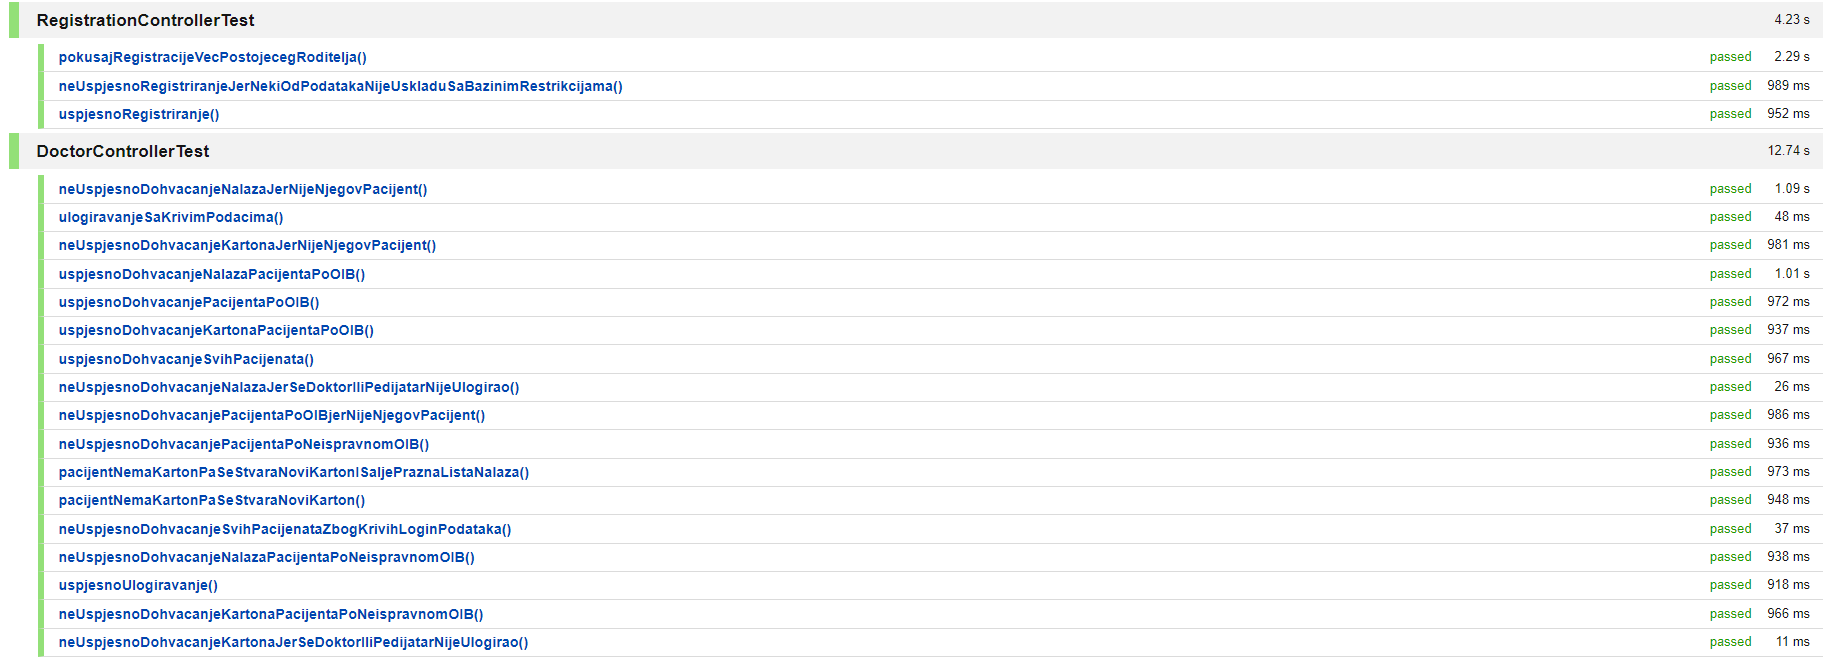
\includegraphics[scale=0.3]{slike/testoviRazreda.PNG} %veličina slike u odnosu na originalnu datoteku i pozicija slike
				\centering
				\caption{Prikaz izvršenih testova}
				\label{fig:slikatestova}
			\end{figure}
			
			\begin{packed_enum}
				
				\item \textbf{Test registracije postojećeg roditelja:}
				\text U navedenom testu šalje se zahtjev za stvaranjem novog entiteta roditelja koji ima već korišteni OIB unutar aplikacije. Očekuje se odgovor tipa "400 Bad Request", kakav odgovor je i dobiven.
				%unos slike
				\begin{figure}[H]
					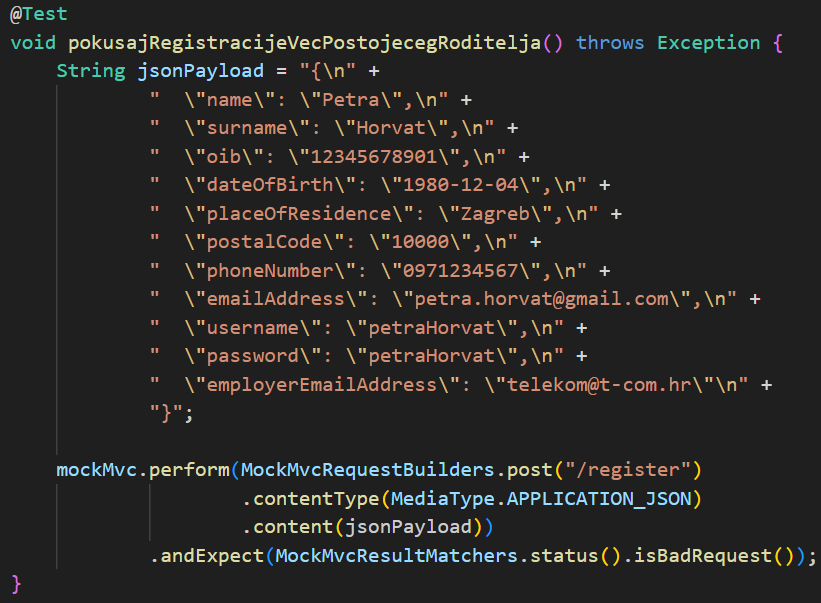
\includegraphics[scale=0.6]{slike/isjecak1.PNG} %veličina slike u odnosu na originalnu datoteku i pozicija slike
					\centering
					\caption{Test registracije postojećeg OIB-a}
					\label{fig:isjecak1}
				\end{figure}
				\item \textbf{Test registracije roditelja:}
				\text U navedenom testu šalje se zahtjev za stvaranjem novog entiteta roditelja, i kojemu su svi podaci ispravni. Očekuje se odgovor tipa "200 OK", kakav je i dobiven.
				%unos slike
				\begin{figure}[H]
					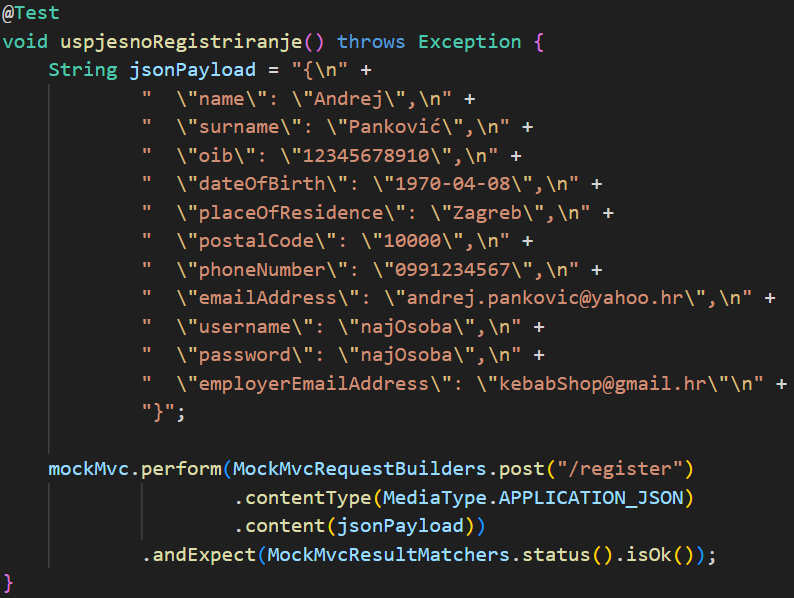
\includegraphics[scale=0.6]{slike/isjecak2.PNG} %veličina slike u odnosu na originalnu datoteku i pozicija slike
					\centering
					\caption{Test registracije roditelja}
					\label{fig:isjecak2}
				\end{figure}
				\item \textbf{Test prijave i dobavljanja svih pacijenata:}
				\text U navedenom testu šalju se ispravni podaci za prijavu, nakon čega se šalje zahtjev za popisom svih pacijenata prijavljenog doktora. Očekuje se odgovor tipa "200 OK", kakav je i dobiven.
				%unos slike
				\begin{figure}[H]
					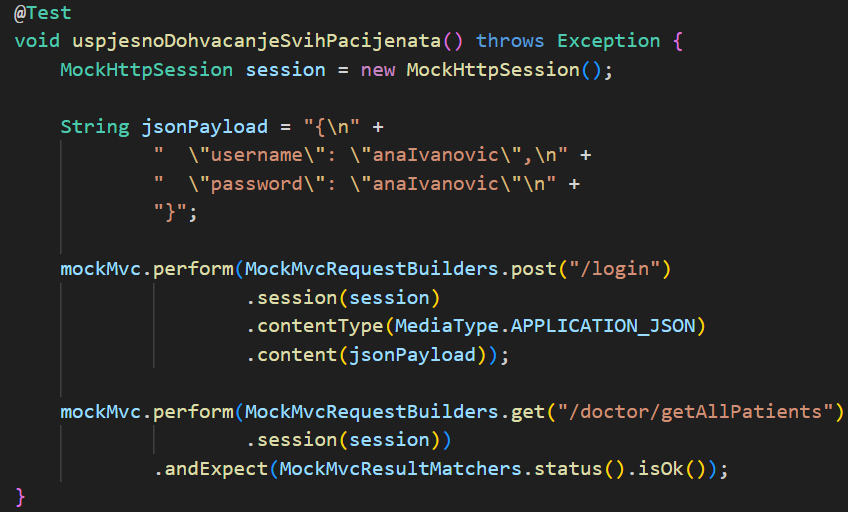
\includegraphics[scale=0.6]{slike/isjecak3.PNG} %veličina slike u odnosu na originalnu datoteku i pozicija slike
					\centering
					\caption{Test dobavljanja pacijenata}
					\label{fig:isjecak3}
				\end{figure}
				\item \textbf{Test dobavljanja kartona:}
				\text U navedenom testu šalju se ispravni podaci za prijavu, nakon čega se šalje zahtjev za kartonom određenog pacijenta. Taj pacijent nema postojeći karton, te je potrebno stvoriti novi. Očekuje se odgovor tipa "200 OK", kakav je i dobiven.
				%unos slike
				\begin{figure}[H]
					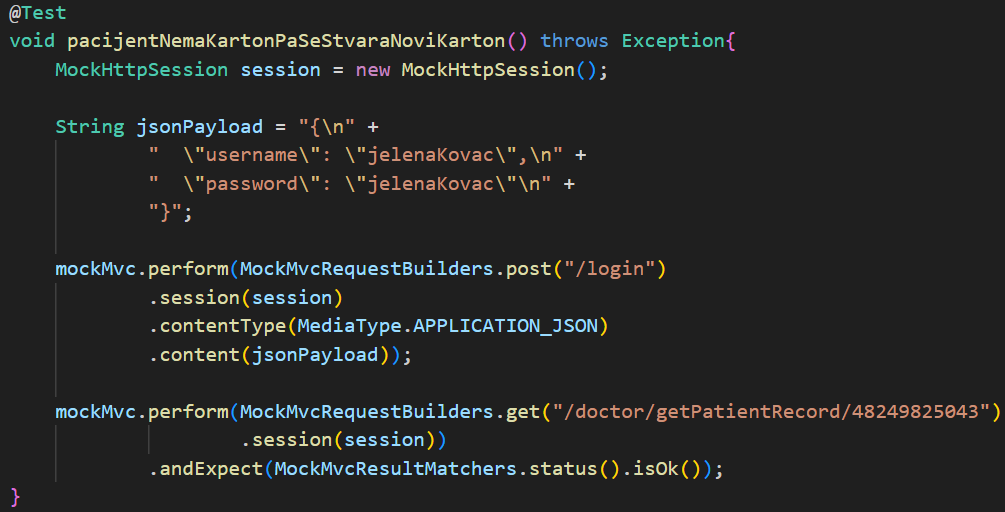
\includegraphics[scale=0.6]{slike/isjecak4.PNG} %veličina slike u odnosu na originalnu datoteku i pozicija slike
					\centering
					\caption{Test dobavljanja kartona}
					\label{fig:isjecak4}
				\end{figure}
				\item \textbf{Test dobavljanja pacijenta po neispravnom OIB-u:}
				\text U navedenom testu šalju se ispravni podaci za prijavu, nakon čega se šalje zahtjev za profilom pacijenta čiji OIB nije unesen u sustav. Očekuje se odgovor tipa "400 Bad Request", kakav je i dobiven.
				%unos slike
				\begin{figure}[H]
					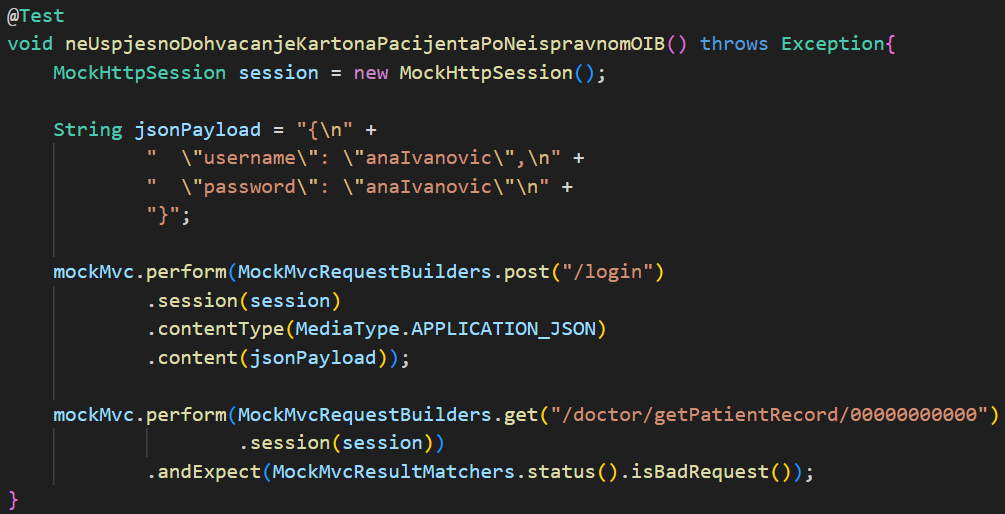
\includegraphics[scale=0.6]{slike/isjecak5.PNG} %veličina slike u odnosu na originalnu datoteku i pozicija slike
					\centering
					\caption{Test dobavljanja pacijenata s neispravnim OIB-om}
					\label{fig:isjecak5}
				\end{figure}
				\item \textbf{Test dobavljanja nalaza pacijenta:}
				\text U navedenom testu šalju se ispravni podaci za prijavu, nakon čega se šalje zahtjev za nalazima pacijenta prijavljenog doktora. Očekuje se odgovor tipa "200 OK", kakav je i dobiven.
				%unos slike
				\begin{figure}[H]
					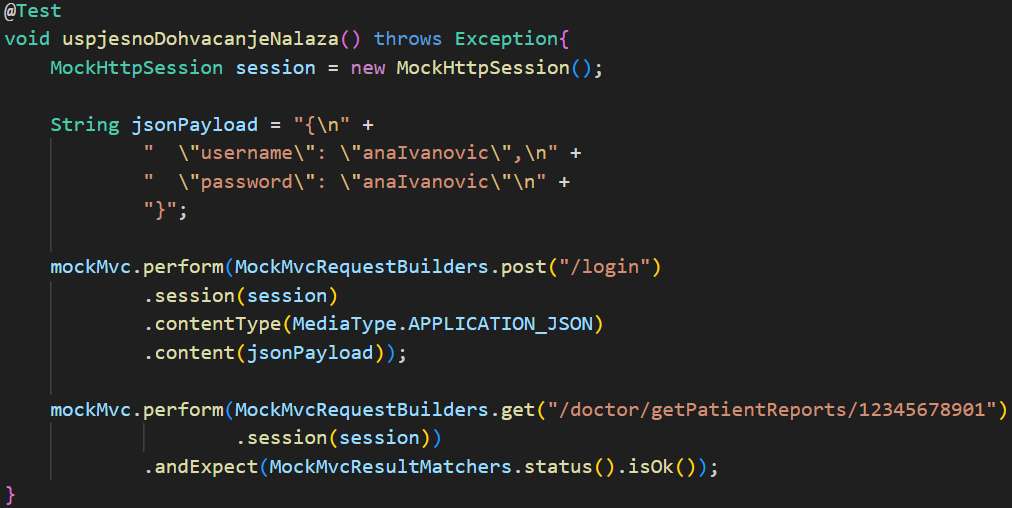
\includegraphics[scale=0.6]{slike/isjecak6.PNG} %veličina slike u odnosu na originalnu datoteku i pozicija slike
					\centering
					\caption{Test dobavljanja nalaza}
					\label{fig:isjecak6}
				\end{figure}
				
			\end{packed_enum}
			\clearpage
			
			
			\subsection{Ispitivanje sustava}
			
			 Ispitivanje sustava provedeno je pomoću alata Selenium IDE, koji se koristi kao dodatak na preglednik, u našem slučaju dodatak na Google Chrome. U nastavku su opisani testni slučajevi.
			 \begin{enumerate}
			 	\item \textbf{\textit{Login} test} - Prvi test sustava bio je provjera uspješne prijave korisnika u sustav. Očekivani izlaz je uspješno provedena prijava i preusmjeravanje na početnu stranicu za korisnike. Na slikama 5.8 i 5.9 prikazani su unosi i rezultati testa.
			 	%unos slike
			 	\begin{figure}[H]
			 		\includegraphics[scale=0.3]{slike/testSustava1.PNG} %veličina slike u odnosu na originalnu datoteku i pozicija slike
			 		\centering
			 		\caption{Unosi za prvi test}
			 		\label{fig:testsustava1}
			 	\end{figure}
			 	%unos slike
			 	\begin{figure}[H]
			 		\includegraphics[scale=0.6]{slike/testSustava2.PNG} %veličina slike u odnosu na originalnu datoteku i pozicija slike
			 		\centering
			 		\caption{Rezultati prvog testa}
			 		\label{fig:testsustava2}
			 	\end{figure}
			 	\clearpage
			 	\item \textbf{Registracija pa \textit{login} test} - Drugi test sustava bio je provjera uspješne registracije, i zatim prijave s istim korisničkim računom. Očekivani izlaz je uspješno provedena prijava i preusmjeravanje na početnu stranicu za korisnike. Na slikama 5.10 i 5.11 prikazani su unosi i rezultati testa.
			 	%unos slike
			 	\begin{figure}[H]
			 		\includegraphics[scale=0.3]{slike/testSustava4.PNG} %veličina slike u odnosu na originalnu datoteku i pozicija slike
			 		\centering
			 		\caption{Unosi za drugi test}
			 		\label{fig:testsustava3}
			 	\end{figure}
			 	%unos slike
			 	\begin{figure}[H]
			 		\includegraphics[scale=0.6]{slike/testSustava3.PNG} %veličina slike u odnosu na originalnu datoteku i pozicija slike
			 		\centering
			 		\caption{Rezultati drugog testa}
			 		\label{fig:testsustava4}
			 	\end{figure}
			 	\clearpage
			 	\item \textbf{Pristup podacima pacijenta test} - Treći test sustava bio je provjera uspješne prijave, i pristupa profilu pacijentu. Očekivani izlaz je uspješno provedena prijava i preusmjeravanje na početnu stranicu za liječnika, gdje se odabire pacijent. Na slikama 5.12 i 5.13 prikazani su unosi i rezultati testa.
			 	%unos slike
			 	\begin{figure}[H]
			 		\includegraphics[scale=0.3]{slike/testSustava6.PNG} %veličina slike u odnosu na originalnu datoteku i pozicija slike
			 		\centering
			 		\caption{Unosi za treći test}
			 		\label{fig:testsustava5}
			 	\end{figure}
			 	%unos slike
			 	\begin{figure}[H]
			 		\includegraphics[scale=0.6]{slike/testSustava5.PNG} %veličina slike u odnosu na originalnu datoteku i pozicija slike
			 		\centering
			 		\caption{Rezultati trećeg testa}
			 		\label{fig:testsustava6}
			 	\end{figure}
			 	\clearpage
			 	
			 	\item \textbf{Dodavanje nove dijagnoze} - Četvrti test sustava bio je provjera uspješne prijave, i pristupa profilu pacijentu. Nakon toga potrebno je otvoriti prozor za dodavanje nove dijagnoze, i njen unos. Očekivani izlaz je uspješno dodana dijagnoza u prozoru liječničkog kartona. Na slikama 5.14 i 5.15 prikazani su unosi i rezultati testa.
			 	%unos slike
			 	\begin{figure}[H]
			 		\includegraphics[scale=0.3]{slike/testSustava8.PNG} %veličina slike u odnosu na originalnu datoteku i pozicija slike
			 		\centering
			 		\caption{Unosi za četvrti test}
			 		\label{fig:testsustava7}
			 	\end{figure}
			 	%unos slike
			 	\begin{figure}[H]
			 		\includegraphics[scale=0.6]{slike/testSustava7.PNG} %veličina slike u odnosu na originalnu datoteku i pozicija slike
			 		\centering
			 		\caption{Rezultati četvrtog testa}
			 		\label{fig:testsustava8}
			 	\end{figure}
			 \end{enumerate}
			\eject 
		
		
		\section{Dijagram razmještaja}
			
			\text Dijagrami razmještaja spadaju pod strukturne i statičke UML dijagrame koji opisuju topologiju sustava, te su usredotočeni na odnos sklopovskih i programskih dijelova. Na slici 5.X prikazan je dijagram razmještaja naše aplikacije. Na klijentskom se računalu nalazi web preglednik kojim se putem HTTPS veze pristupa aplikaciji. Web aplikacija pokrenuta je unutar web poslužitelja, koji se nalazi na poslužiteljskom računalu. Unutar okoline izvođenja web poslužitelja također se nalazi i baza podataka. Razlog manjku zasebnog poslužitelja za bazu podataka je korištenje baze H2, koja je integrirana u \textit{backend}.
			
			%unos slike
			\begin{figure}[H]
				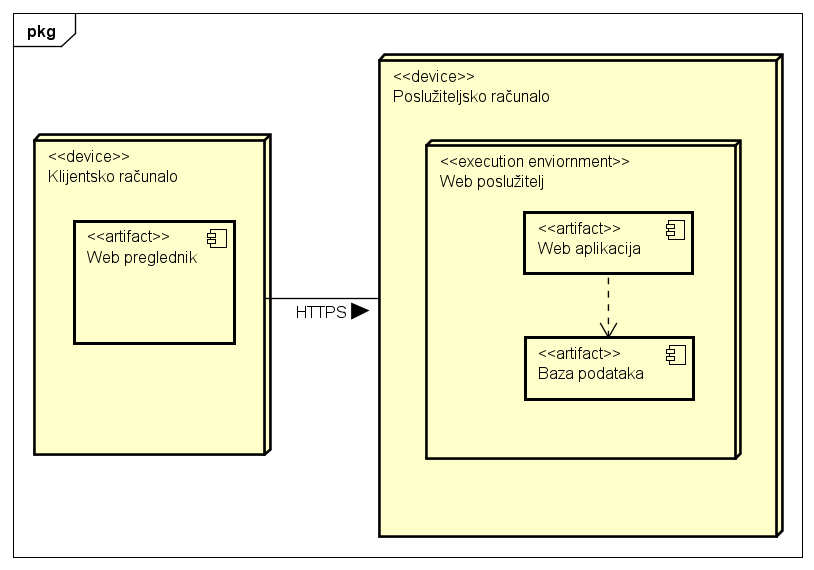
\includegraphics[scale=0.7]{dijagrami/dijrazm1.PNG} %veličina slike u odnosu na originalnu datoteku i pozicija slike
				\centering
				\caption{Dijagram razmještaja}
				\label{fig:dijstanj1}
			\end{figure}
			
			\eject 
		
		\section{Upute za puštanje u pogon}
		
			\subsection{\textit{Deploy} na Render - Backend}
			Potrebno je postaviti izvorni kod aplikacije na vlastiti repozitorij na servisu GitHub. Izvorni kod moguće je preuzeti s GitHub repozitorija projekta, čija se poveznica nalazi u literaturi. Jednom kada je cijeli izvorni kod na repozitoriju, potrebno je otvoriti stranicu servisa Render\footnote{https://dashboard.render.com/}, te se prijaviti ili kreirati račun. Kada je prijava provedena, potrebno je odabrati opciju "New", te odabrati opciju \textit{Web service}.
				%unos slike
			\begin{figure}[H]
				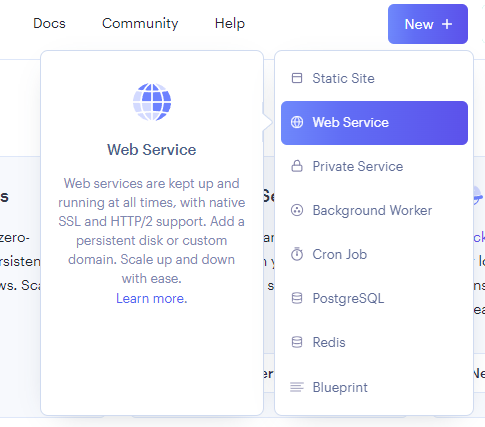
\includegraphics[scale=0.9]{slike/render0.PNG} %veličina slike u odnosu na originalnu datoteku i pozicija slike
				\centering
				\caption{Opcija \textit{Web service}}
				\label{fig:render0}
			\end{figure}
			Nakon toga, potrebno je odabrati prvu opciju na sljedećem izborniku, \textit{Build and deploy from a Git repository}.
			%unos slike
			\begin{figure}[H]
				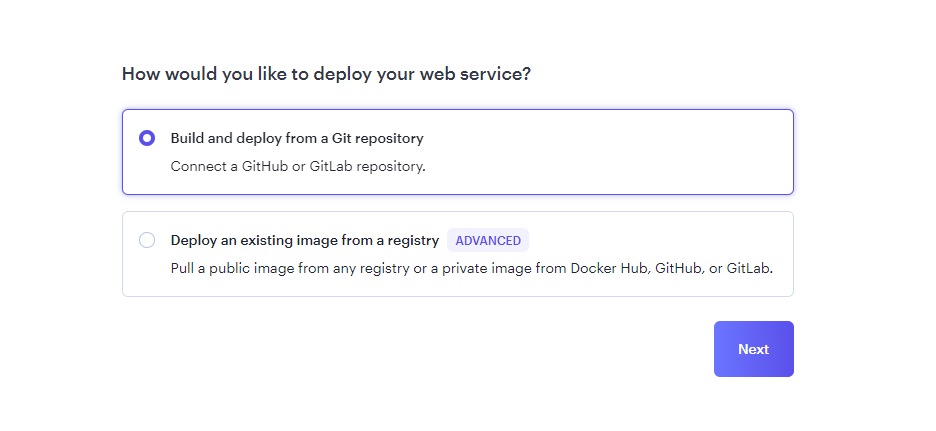
\includegraphics[scale=0.7]{slike/render1.PNG} %veličina slike u odnosu na originalnu datoteku i pozicija slike
				\centering
				\caption{Izbornik za \textit{deploy}}
				\label{fig:render1}
			\end{figure}
			Na idućem ekranu potrebno je prijaviti se pomoću svog GitHub ili GitLab računa. Nakon što se korisnik uspješno prijavi, nudi mu se lista mogućih repozitorija za dodavanje na Render.
			%unos slike
			\begin{figure}[H]
				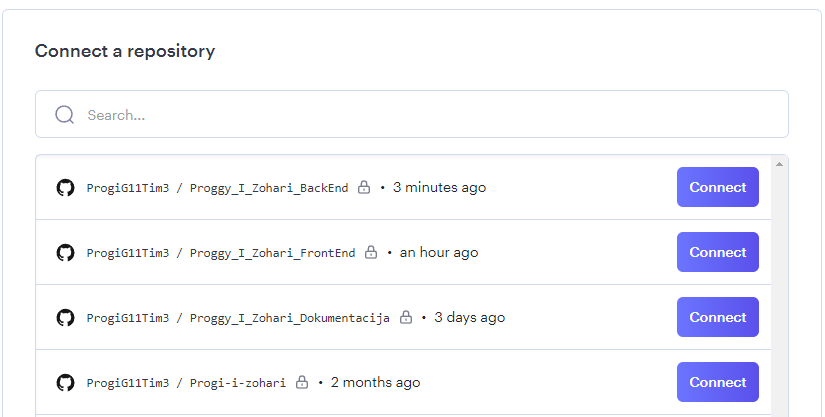
\includegraphics[scale=0.7]{slike/render2.PNG} %veličina slike u odnosu na originalnu datoteku i pozicija slike
				\centering
				\caption{Izbornik repozitorija}
				\label{fig:render2}
			\end{figure}
			Na sljedećem ekranu potrebno je unijeti ime servisa, regiju za korištenje, izvorni/korijenski direktorij te \textit{Runtime} opciju. Pod pretpostavkom da je odabran direktorij za \textit{backend}, unesene opcije trebaju biti sljedeće:
			%unos slike
			\begin{figure}[H]
				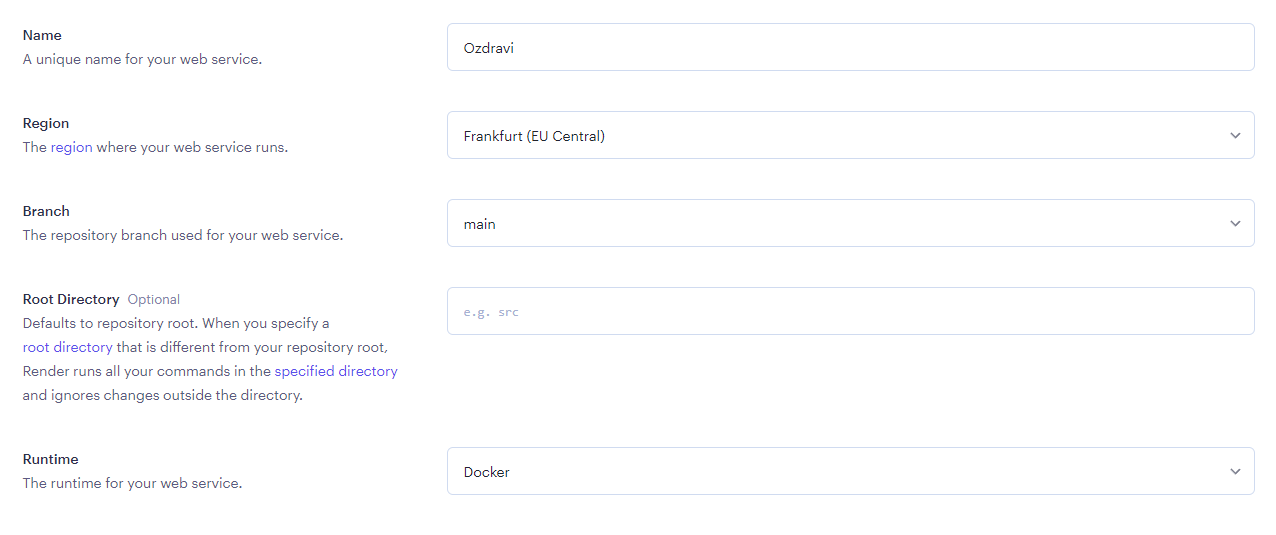
\includegraphics[scale=0.7]{slike/render3.PNG} %veličina slike u odnosu na originalnu datoteku i pozicija slike
				\centering
				\caption{Izbornik opcija za stvaranje \textit{backenda}}
				\label{fig:render3}
			\end{figure}
			Dodatno, potrebno je otvoriti opciju \textit{Advanced} te unijeti putanju do \textit{Dockerfile}, što se u slučaju aplikacije ozdravi nalazi na lokaciji \textbf{./docker/Dockerfile}:
			%unos slike
			\begin{figure}[H]
				
\includegraphics[scale=0.7]{slike/render4.PNG} %veličina slike u odnosu na originalnu datoteku i pozicija slike
				\centering
				\caption{Unos lokacije Dockerfilea}
				\label{fig:render4}
			\end{figure}
			Potrebno je još samo stisnuti gumb \textit{Create Web Service}. \clearpage
			\eject
			
			\subsection{\textit{Deploy} na Render - Frontend}
			Za \textit{deploy} \textit{frontend} dijela aplikacije, potrebno je ponovno odabrati opcije \textbf{New - Web service}. Prilikom unosa opcija, ovaj puta se postupa malo drugačije. Potrebno je unijeti naziv, te dodati \textbf{frontend} kao \textit{root directory}, a zatim odabrati opciju \textit{Node} unutar opcije \textit{Runtime}. Uz to, potrebno je unijeti komandu \textbf{yarn build} unutar opcije \textit{Build Command} i \textbf{yarn start-prod} unutar \textit{Start Command}. 
			%unos slike
			\begin{figure}[H]
				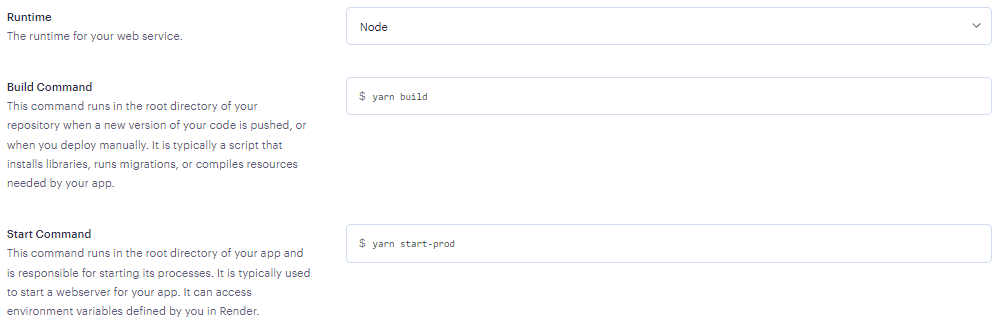
\includegraphics[scale=0.8]{slike/render5.PNG} %veličina slike u odnosu na originalnu datoteku i pozicija slike
				\centering
				\caption{Unos opcija za \textit{frontend}}
				\label{fig:render5}
			\end{figure}
			Potrebno je još samo otvoriti opciju \textit{Advanced}, te u dodatne \textit{environment} varijable dodati varijablu imena\textbf{ API\textunderscore BASE\textunderscore URL}, te postaviti \textit{value} na adresu deployanog backenda aplikacije dostupnu na Render dashboardu.
			%unos slike
			\begin{figure}[H]
				
\includegraphics[scale=0.8]{slike/render6.PNG} %veličina slike u odnosu na originalnu datoteku i pozicija slike
				\centering
				\caption{Unos opcije za povezivanje}
				\label{fig:render6}
			\end{figure}
			Ponovno, potrebno je još samo pritisnuti \textit{Create Web Service}.
			
			
			\eject 